\section{Chapter 5 - Problem (15)}
	Block $A$ in the figure has mass $m_{A} = 0.24 \ sl$, and block $B$ has mass $m_{B} = 0.13 \ sl$. The coefficient of kinetic friction between block $B$ and the horizontal plane is $\mu_{k} = 0.45$. The inclined plane is frictionless and at angle $\theta = 36^{o}$. The pulley serves only to change the direction of the cord connecting the blocks. The cord has negligible mass.

	\begin{figure}[H]
		\begin{center}
			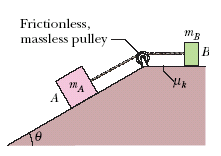
\includegraphics[scale=1]{hw6_problem15}
			\caption{Illustration of Problem 15}
			\label{fig:hw6_problem15}
		\end{center}
	\end{figure}

	\begin{figure}[H]
		\begin{center}
			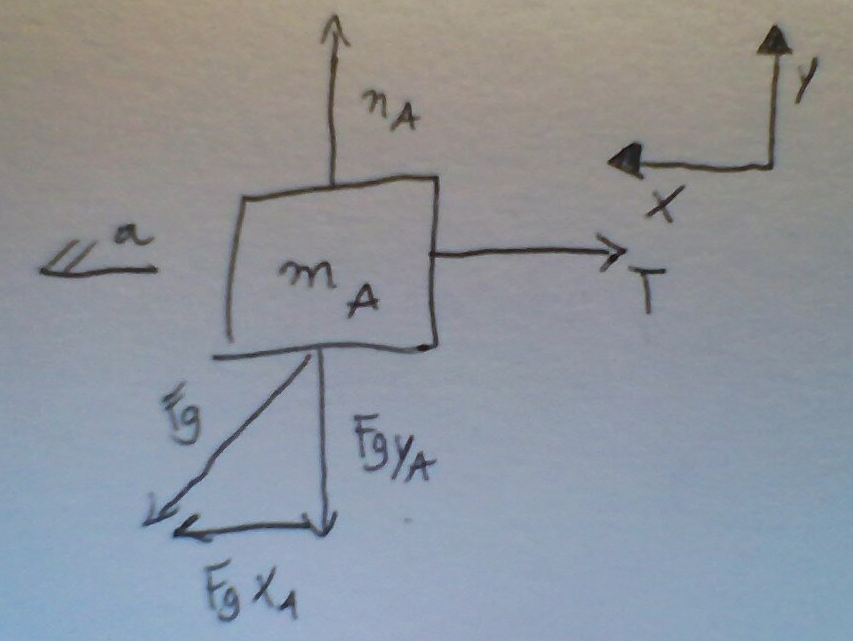
\includegraphics[scale=0.3]{hw6_problemf_ma_fbd}
			\caption{Free-Body Diagram (Problem 15 (Block $A$))}
			\label{fig:hw6_problemf_ma_fbd}
		\end{center}
	\end{figure}

	\begin{figure}[H]
		\begin{center}
			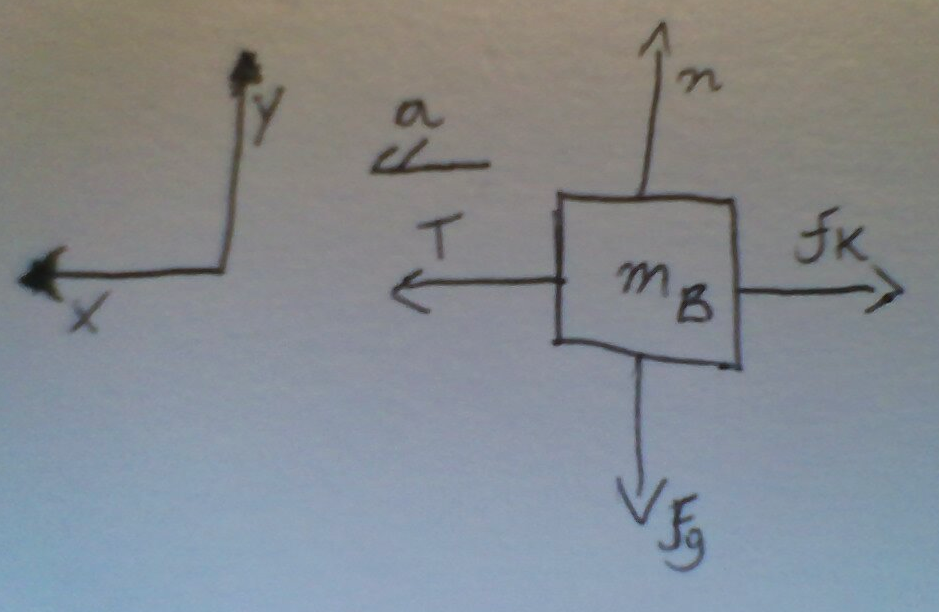
\includegraphics[scale=0.3]{hw6_problemf_mb_fbd}
			\caption{Free-Body Diagram (Problem 15 (Block $B$))}
			\label{fig:hw6_problemf_mb_fbd}
		\end{center}
	\end{figure}

	\subsection{Question (a)}

		Find the tension in the cord:

		\textbf{R:} \newline

		Newton's $2^{nd}$ Law on Block $A$:
		\begin{align}
			\sum F_{x_{A}} = \ &m_{A}a_{x_{A}}& \notag \\
			f_{g_{x_{A}}} - T = \ &m_{A}a& \notag \\
			T = \ &m_{A}g \sin \theta - m_{A}a& \notag
		\end{align}

		\begin{align}
			\sum F_{y_{A}} = \ &m_{A}a_{y_{A}}& \notag \\
			n_{A} - f_{g_{y_{A}}} = \ &m_{A}(0)& \notag \\
			n_{A} = \ &m_{A}g \cos \theta& \notag
		\end{align}

		Newton's $2^{nd}$ Law on Block $B$:
		\begin{align}
			\sum F_{x_{B}} = \ &m_{B}a_{x_{B}}& \notag \\
			T - f_{k} = \ &m_{B}a& \notag \\
			T = \ &m_{B}a + \mu_{k}n_{B}& \notag
		\end{align}

		\begin{align}
			\sum F_{y_{B}} = \ &m_{B}a_{y_{B}}& \notag \\
			n_{B} - f_{g_{y_{B}}} = \ &m_{B}(0)& \notag \\
			n_{B} = \ &m_{B}g& \notag
		\end{align}

		Finding the acceleration:

		\begin{align}
			m_{A}g \sin \theta - m_{A}a = \ &m_{B}a + \mu_{k}n_{B}& \notag \\
			m_{A}a + m_{B}a = \ &m_{A}g \sin \theta - \mu_{k}n_{B}& \notag \\
			a = \ &\frac{m_{A}g \sin \theta - \mu_{k}n_{B}}{m_{A} + m_{B}}& \notag
		\end{align}

		\begin{align}
			m_{A}g \sin 36^{o} = \ &(0.24 \ sl)\left(32.2 \ ft/s^{2}\right)(0.588)& \notag \\
			= \ &4.542 \ lb& \notag
		\end{align}

		\begin{align}
			\mu_{k}n_{B} = \ &(0.45)m_{B}g& \notag \\
			= \ &(0.45)(0.13 \ sl)\left(32.2 \ ft/s^{2}\right)& \notag \\
			= \ &1.884 \ lb& \notag
		\end{align}

		\begin{align}
			a = \ &\frac{m_{A}g \sin \theta - \mu_{k}n_{B}}{m_{A} + m_{B}}& \notag \\
			= \ &\frac{(4.542 \ lb) - (1.884 \ lb)}{(0.24 \ sl) + (0.13 \ sl)}& \notag \\
			= \ &\frac{2.658 \ lb}{0.37 \ sl}& \notag \\
			= \ &7.184 \ ft/s^{2}&
			\label{eq:hw6_f_acc}
		\end{align}

		Finding the tension:

		\begin{align}
			T = \ &m_{A}g \sin \theta - m_{A}a& \notag \\
			T = \ &(4.642 \ lb) - (0.24 \ sl)\left(7.184 \ ft/s^{2}\right)& \notag \\
			T = \ &(4.642 \ lb) - (1.724 \ lb)& \notag \\
			T = \ &2.918 \ lb&
		\end{align}

	\subsection{Question (b)}

		Find the magnitude of the acceleration of the blocks:

		\textbf{R:} \newline

		As seen on \cref{eq:hw6_f_acc}:
		\begin{align}
			a = \ &7.184 \ ft/s^{2}& \notag
		\end{align}
